\subsection{Sơ đồ thực thể liên kết (ERD)}

\begin{figure}[H]
    \centering
    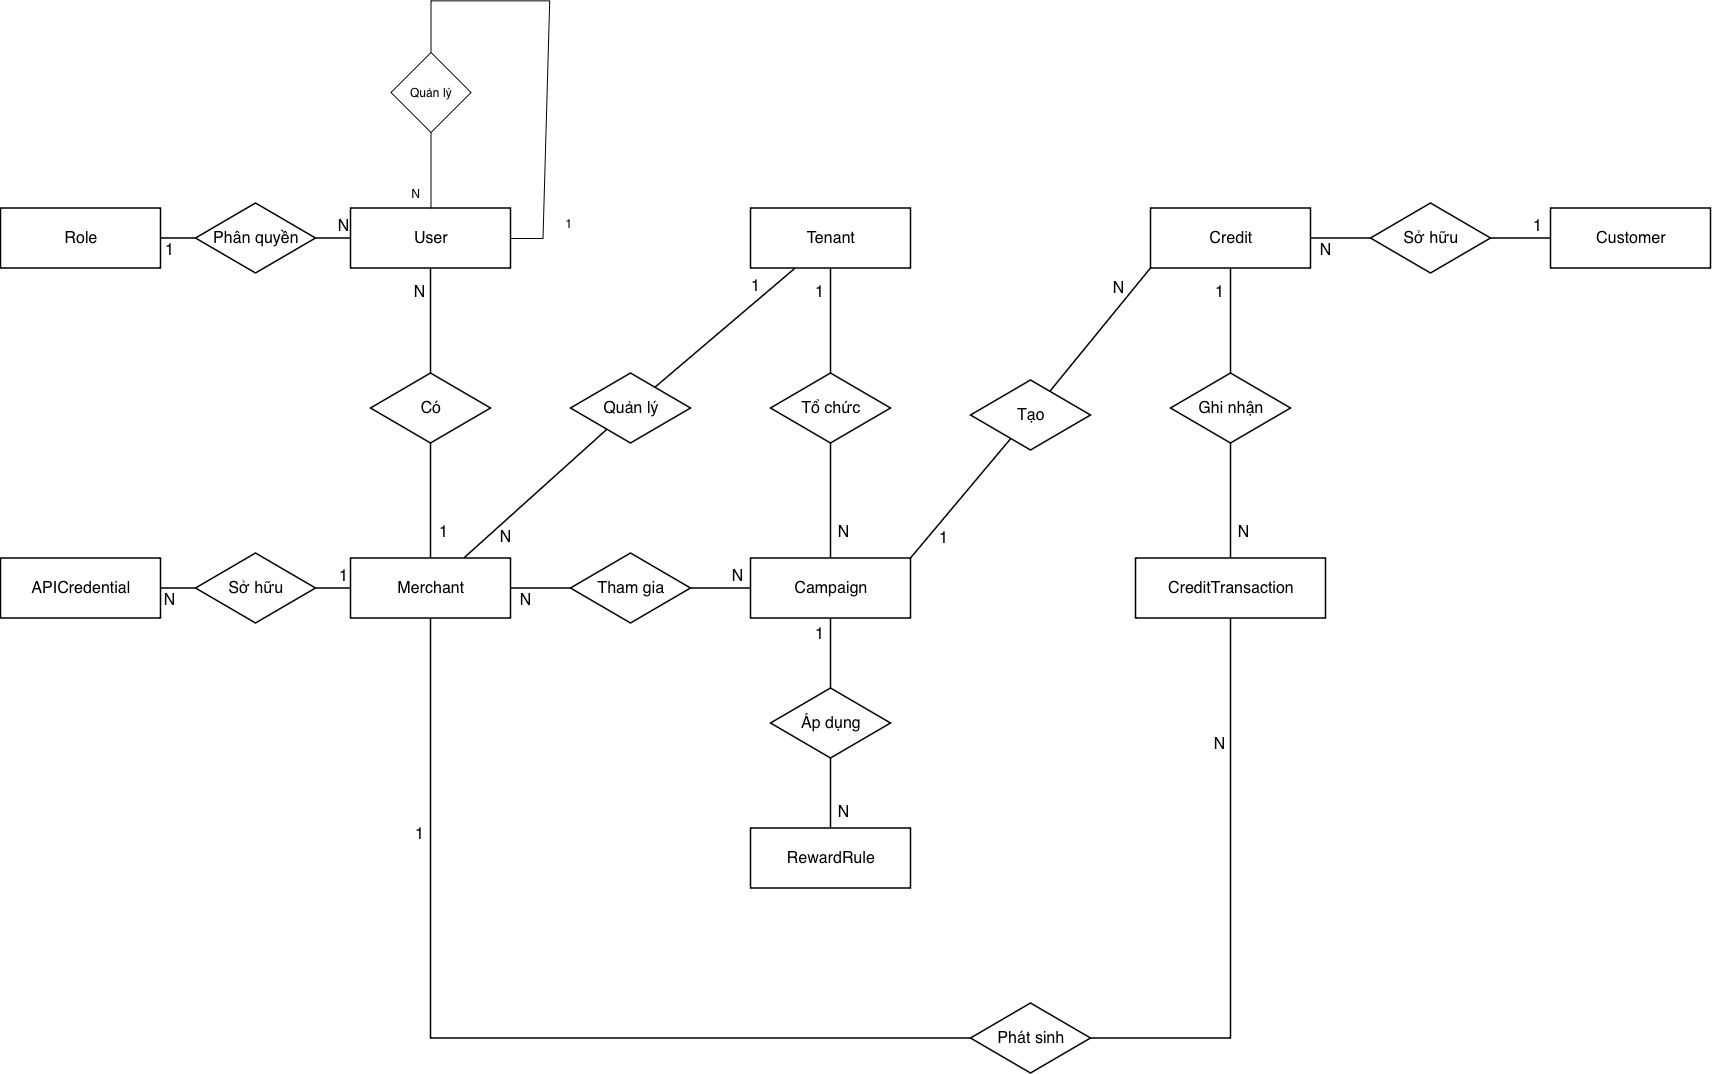
\includegraphics[width=\textwidth]{images/conceptual_diagram.jpg}
    \caption{Sơ đồ thiết kế quan niệm (Conceptual Diagram)}
    \label{fig:conceptual_diagram}
\end{figure}
% =========================================================
% TÙY CHỌN 2: CHÈN ẢNH DRAW.IO (KHI NÀO VẼ XONG THÌ DÙNG)
% Hướng dẫn:
% 1. Xóa (hoặc bôi đen nhấn Ctrl + /) toàn bộ đoạn code \begin{figure} của Tùy chọn 1 ở trên.
% 2. Xóa các dấu % ở đầu các dòng code của phần Tùy chọn 2 bên dưới để kích hoạt.
% 3. Lưu ảnh ERD tải về từ draw.io vào thư mục images/ với tên erd_quan_niem.png
% =========================================================

% \begin{figure}[H]
%     \centering
%     \includegraphics[width=0.95\textwidth]{images/erd_quan_niem.png}
%     \caption{Sơ đồ Thực thể Kết hợp (ERD) mức quan niệm hệ thống OctaPoint CaaS}
%     \label{fig:erd_drawio}
% \end{figure}
CreditTransaction có khóa TransactionID riêng nên là thực thể mạnh, dù phụ thuộc tồn tại vào Credit. Quan hệ Ghi nhận không phải quan hệ định danh của thực thể yếu. Các nhãn 0..1 biểu diễn người quản lý và chiến dịch tùy chọn; mỗi cặp Customer--Merchant có tối đa một Credit.
